\chapter{Proposed approach}

In the previous chapter, a review of two splicing detection methods based on illuminant colors analysis has been presented. However, their effectiveness still need to be improved for real forensic applications.

The approach proposed in this chapter has been developed to correct some of the two approaches drawbacks and mainly to combine them together in order to realize a more general algorithm for image forgery detection. 

\section{Overview}

Most of the times, the splicing detection process relies on the expert's experience and background knowledge. This process usually is time consuming and error prone once that image splicing is more and more sophisticated and an aural (e.g., visual) analysis may not be enough to detect forgeries.

This approach to detecting image splicing is developed aiming at minimizing the user interaction. 

The two methods, presented in the previous chapter \cite{carvalho2016illuminant} and \cite{fan2015image}, are now being used in synergy with each other, going to analyze the suspicious image and at the same time looking for potential signs of forgery.

Starting from an image we want to analyze, the method will output a set of results.
\begin{itemize}
\item A classification \textbf{label} indicating whether an image is believed to be original or counterfeit.
\item A classification \textbf{score} indicating the confidence of the algorithm output.
\item A \textbf{detection map} highlighting the detected spliced regions.
\end{itemize}

The proposed approach minimizes the needed human interaction and aims at being a fully automated process. However, not both the modules can operate in any circumstance. The face splicing detection module works only if there is a number of faces greater than or equal to two.

\section{Face splicing detection module}

The first module consists in the implementation, with few enhancements and simplifications, of the method proposed by Carvalho et al. \cite{carvalho2016illuminant} and presented in Section 1.6.

The algorithm can be used on an image that contains at least two human faces, looking for inconsistencies in the illuminant color in presence of human skin. In particular, in case of a forgery detection, the algorithm tries to guess which faces in the images are doctored.

The algorithm requires an initial training phase, so a dataset with annotated human faces is needed. 

This module consists of 4 consecutive stages:

\begin{enumerate}
\item \textbf{Illuminant maps extraction}: given an input image, two different illuminant maps are evaluated, using the IIC and GGE extraction methods.
\item \textbf{Face detection}: after the illuminant maps extraction, the human faces in the image are detected. In the training phase the faces positions are read from the groundtruth file. If the given image contains less than two faces, it is discarded.
\item \textbf{Paired face feature extraction}: human faces are considered and classified in pairs. From each extracted face in the previous step, a color descriptor is used in order to extract features.
\item \textbf{KNN models training}: fixed a value of $K$, a set of KNN models are trained using previous feature vectors.
\item \textbf{Forgery detection and classification}: in this step an image is classified as fake or normal. Given an image classified as fake, the analysis is refined pointing out which face of the image is the result of a composition.
\end{enumerate}

\subsection{Illuminant maps extraction}

Given a single image $I$ the two different illuminant maps are extracted: both generalized grayworld algorithm (GGE) and inverse-intensity chromaticity estimation (IIC) are used.

\begin{figure}[!htb]
\minipage{0.32\textwidth}
  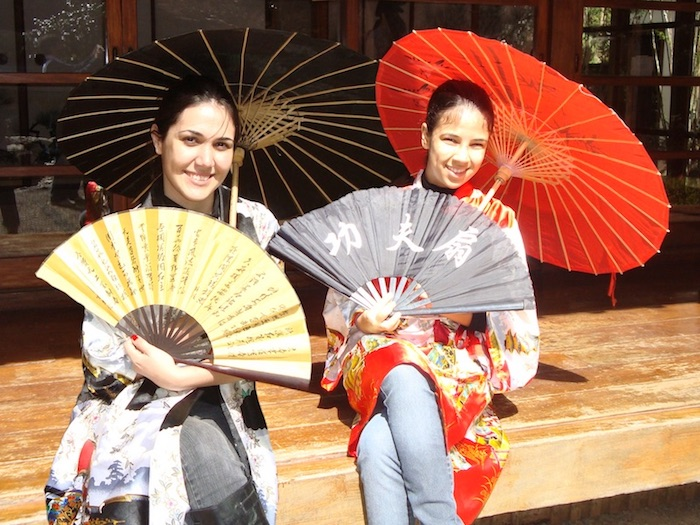
\includegraphics[width=\linewidth]{splicing-33.jpg}
  \caption{The original image}\label{fig:awesome_image1}
\endminipage\hfill
\minipage{0.32\textwidth}
  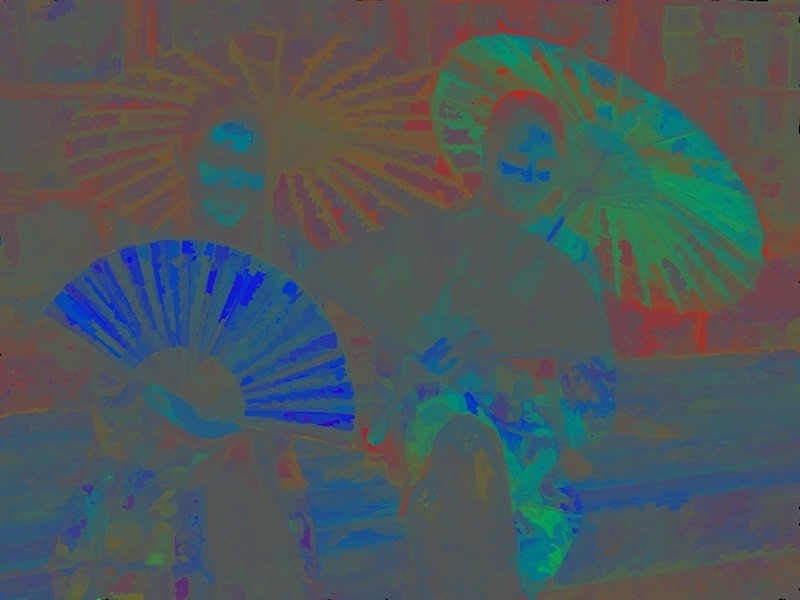
\includegraphics[width=\linewidth]{splicing-33_gge_map.jpg}
  \caption{GGE illuminant map}\label{fig:awesome_image2}
\endminipage\hfill
\minipage{0.32\textwidth}%
  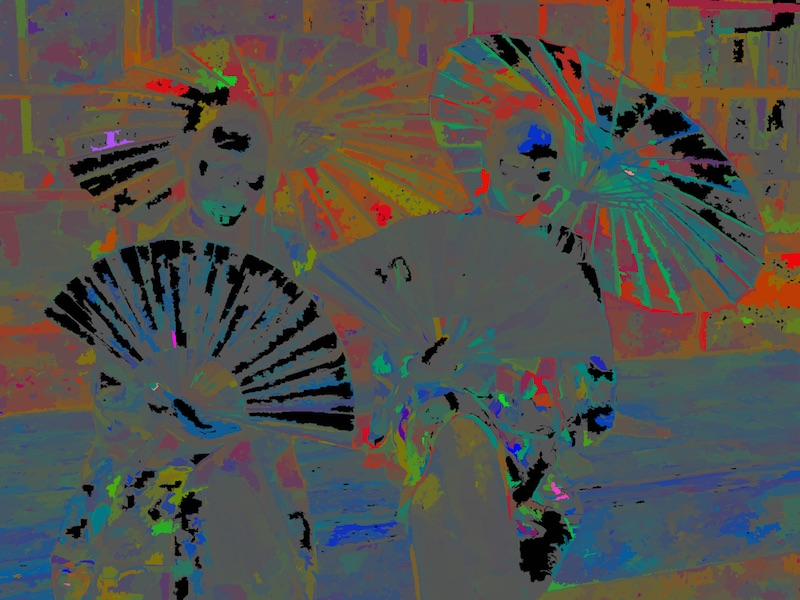
\includegraphics[width=\linewidth]{splicing-33_iic_map.jpg}
  \caption{IIC illuminant map}\label{fig:awesome_image3}
\endminipage
\end{figure}

Differently from de Carvalho et al. \cite{carvalho2016illuminant}, who have used the conversion of IMs to the YCbCr color space, the two IMs are considered as two different color maps theirself.

The illuminant maps extraction algorithm implementation used is the one proposed by Riess et. al. for \cite{riess2010scene} and downloadable in the project page\footnote{Homepage of the project \cite{riess2010scene} - www5.cs.fau.de/research/areas/computer-vision/image-forensics/scene-illumination-as-an-indicator-of-image-manipulation}. The code provides an implementation of both of the two illuminant map extraction methods, using a local estimation approach.

\subsection{Face detection}

One of the drawback of the method proposed by Carvalho et al. \cite{carvalho2016illuminant} relies on the user interaction needed for detecting human faces in the image. In this approach a common face detection module is used to achieve the same results, aiming at minimizing the user dependency and making the entire algorithm user independent.

The face detector used is the one initially proposed by Viola and Jones \cite{viola2001rapid}\cite{viola2004robust} and improved by Lienhart et al. \cite{lienhart2002extended}. Usually called simply \emph{Viola-Jones}, its original motivation was face detection, but it can be trained to detect different object classes. 

This detector combines four key concepts: 
\begin{itemize}
\item Simple rectangular features, called \emph{Haar features}
\item \emph{Integral Image}\cite{crow1984summed} concept for rapid feature detection 
\item \emph{AdaBoost}\cite{freund1995desicion} machine-learning method 
\item A \emph{cascade classifier} to combine all features efficiently 
\end{itemize}

The used rectangle combinations are not true \emph{Haar wavelets}\cite{haar1910theorie}. Instead, they contain better suited rectangle combinations used for visual object detection. The presence of an Haar feature is determined by subtracting the pixel values of the dark region from the pixel values of the light one. If the difference exceeds a threshold value set during the training process, the feature is said to be present. 

\begin{figure}[h!]
  \centering
    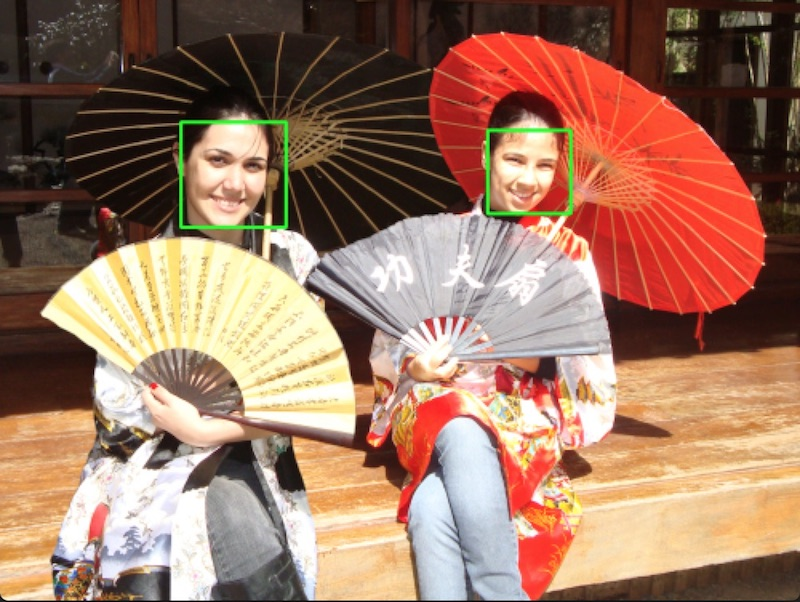
\includegraphics[width=0.5\textwidth]{facedetected}
    \caption{The output of the Viola and Jones face detector}
    \label{fig:facesdetected}
\end{figure}

\emph{OpenCV}\footnote{OpenCV - Open source computer vision. http://opencv.org} provides an implementation of the Viola-Jones face detector as \emph{cvHaarDetectObjects}.

Figure \ref{fig:facesdetected} shows the output of the face detector module. Given the output faces bounding boxes, the corresponding regions in the illuminant maps are extracted, Figure \ref{fig:facesdetectedmaps}.

\begin{figure}[h!]
  \centering
    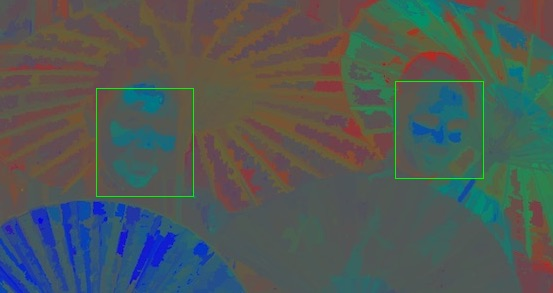
\includegraphics[width=0.5\textwidth]{splicing-33_gge_map_faces}
    \caption{The extracted faces from illuminant map}
    \label{fig:facesdetectedmaps}
\end{figure}

\subsection{Paired face feature extraction}

From each extracted face in the previous step, we need to find telltales that allow identification of spliced images. 

According to Riess and Angelopoulou \cite{riess2010scene}, when the output illumination maps are analyzed by an expert for detecting forgeries, the main observed feature is color. Thus, differently from Carvalho et al. \cite{carvalho2016illuminant} who have explored a large set of descriptors of different visual properties (e.g., texture, shape, color, among others) we focused our attention on color descriptors.

The considered color description techniques are ACC \cite{huang1997image}, BIC \cite{stehling2002compact}, CCV \cite{pass1997comparing}, and LCH \cite{swain1991color}.

\subsubsection{ACC descriptor}

\emph{Color Autocorrelogram (ACC) }\cite{huang1997image} maps the spatial information of colors by pixels correlations in different distances. Let $I$ an image, the \emph{autocorrelogram} (the term \emph{“correlogram”} is adapted from spatial data analysis \cite{upton1985spatial}) computes the probability of finding two pixels in $I$ with a color $c$ in a distance $d$ from each other. 

After the autocorrelogram computation, a set of $m$ probability values for each distance $d$ are considered, where $m$ stands for the number of colors in the quantized space. 

The implemented version quantized the RGB color space into 64 bins and considered 4 distance values (1, 3, 5, and 7). The \emph{L1} distance function is used.

\subsubsection{BIC descriptor}

\emph{Border/Interior Pixel Classification (BIC)} \cite{stehling2002compact} is a region-based color descriptor. Its extraction algorithm classifies the image pixels in border or interior
pixels. 

The image is first quantized into 64 colors in RGB color space. Then, each pixel is classified as interior
if its neighbors (above, below, left and right pixels) have the same color. Otherwise it is classified as border pixel. After the classification, two histograms are generated: one for border pixels and another for interior pixels. These histograms are stored as one single histogram with 128 bins.

\subsubsection{CCV descriptor}

\emph{Color Coherence Vector (CCV)} \cite{pass1997comparing} is a very popular color descriptor in the literature. Its extraction algorithm classifies the image pixels in coherent or incoherent pixels. This classification considers if the pixel belongs or not to a region with similar colors, called \emph{coherent region}. After the classification, two color histograms are computed: one for coherent pixels and another for incoherent pixels.

Both histograms are concatenated to compose the final feature vector. The RGB color space is quantized into 64 bins and L1 distance function is used.

\subsubsection{LCH descriptor}

\emph{Local Color Histogram (LCH)} \cite{swain1991color} is one of the most popular descriptors that is based on fixed size regions to describe image properties. Its extraction algorithm splits the image into fixed size blocks and computes a color histogram for each region. After that, the histograms of each region
are concatenated to compose one single histogram. 

The implemented version splits the image
in 16 regions (4x4 grid) and quantized the RGB color space into 64 bins. This generated feature vectors with 1024 values. The L1 distance function is used.


\subsubsection{Paired features}

In order to detect a face forgery, we need to compare the current analyzed image region (i.e. the current face) against another one, looking for color inconsistencies. Thus, instead of considering each face separately, faces are encoded in pairs.

Given two face feature vectors of the same type (i.e. extracted with the same color descriptor), $\mathcal{D}_1$ and $\mathcal{D}_2$, whose length depends on the color descriptor used, the final descriptor is computed concatenating them into a single feature vector $\mathcal{P}$. So, in an image $I$ containing $q$ faces, a set $S$ of feature vectors are extracted, with

$$
S = \{\mathcal{P}_1, \ldots, \mathcal{P}_m\} \quad \textrm{  where } m = \frac{q (q-1)}{2}
$$

if $q \geq 2$. 

Each paired face descriptor is computed twice for each considered color descriptor, one based on the GGE map and one based on the IIC map.

\subsection{KNN models training}

As in the Carvalho \emph{et al.}\cite{carvalho2016illuminant}, k-Nearest Neighbor (kNN) classifier\cite{bishop2007pattern} are chosen for the classification step.

After the feature vectors are extracted from all faces in the images, a set of 8 \emph{k-nearest neighbors} binary classifiers are trained, 4 models based on the GGE map and 4 based on the IIC map. 

Accordingly to the analysis presented in \cite{carvalho2016illuminant}, the value of $k$ is set to 5.

Given a set of paired feature vectors $\mathcal{P}$, extracted from a new image $I$, each classifier $C_i$ ($i = 1, \ldots, 8$) predicts a label (forgery or real) for these feature vectors, producing $k$ outcomes. All the outcomes are used as input of a fusion technique (in this case, majority voting) that takes the final decision regarding the definition of each paired feature vector $\mathcal{P}$ extracted from $I$.

$$
Score(\mathcal{P}) = \sum_{i = 1}^{8} prediction_{C_i}(\mathcal{P}) \quad \textrm{ where } prediction_{C_i}(\mathcal{P}) \in [0, 1]
$$

Finally, $\mathcal{P}$ is considered as fake if its score is higher than a given threshold. 

An alternative approach for the feature score evaluation has been experimented and presented in Chapter 3.

\subsection{Forgery detection and classification}

Differently from Carvalho \emph{et al.} \cite{carvalho2016illuminant}, we used another approach for classifying the single face as fake using the results of the paired faces classification. 

Let $P_{i, j}$ the paired feature vector computed concatenating the $i$-th and the $j$-th face feature. If $P_{i, j}$ is classified as fake, the scores of the considered images are incremented the prediction output values. At the end of the process, faces with higher associated scores have been classified as fake multiple times.

The resulting scores are then thresholded for selecting the most probably doctored faces. 

Given an input image $I$ containing $q$ faces, the forgery detection algorithm is summarized in Algorithm \ref{alg:faceforgerydetection}.

\begin{algorithm}[!h]
\begin{algorithmic}[1]
\State $Score_i = 0 \qquad \forall i \in Faces$ 
\For {$im \in \{GGE, IIC\}$}
\For {$desc \in \{ACC, BIC, CCV, LCH\}$}
\State $F = extractFeatures(im, desc)$
\State So $F = \{\mathcal{P}_1, \ldots, \mathcal{P}_m\} $ where $ m = \frac{q(q-1)}{2}$
\For {$f \in F$}
\State $prediction = KNN.predict(f)$
\State Let $i, j$ the faces considered for $f$ evaluation
\State Increment $i, j$ scores by $prediction \in [0, 1]$
\EndFor
\EndFor
\EndFor
\For {$i \in Faces$}
\If {$Score_i > Threshold$}
\State Mark $i$ as \emph{fake}
\EndIf
\EndFor
\end{algorithmic}\caption{Face forgery detection}\label{alg:faceforgerydetection}
\end{algorithm}

The output of the detector is a resulting \emph{detection mask}, which highlights the spliced part of the image.

\begin{figure}[h!]
  \centering
    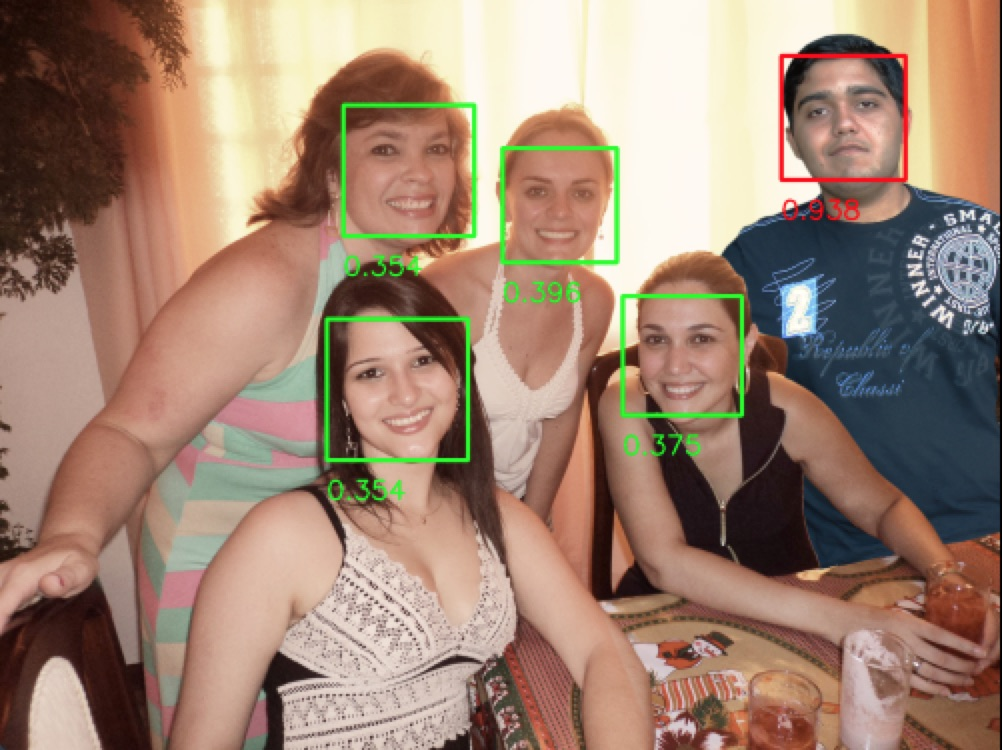
\includegraphics[width=0.8\textwidth]{facedetectionoutput}
    \caption{An example output of the face splicing detection module. Each face is marked in \emph{green} if it has been classified as \emph{normal}, \emph{red} if considered as \emph{fake}. A classification confidence score is presented below each bounding box.}
    \label{fig:facesplicingdetectionoutput}
\end{figure}

An example is shown in Figure \ref{fig:facesplicingdetectionoutput}. Each face is marked as fake or normal and provided of a classification confidence score. The higher the score, the higher the confidence of the prediction output. In the analyzed image (Figure \ref{fig:facesplicingdetectionoutput}), four of the total faces are marked in \emph{green} because they have a low score value. The last face, corresponding to the spliced person, has a very high prediction score and it is therefore marked in \emph{red}.

\section{Region splicing detection module}

The second module is based on the work of Fan \emph{et al.}\cite{fan2015image} (presented in Section 1.7) with some improvements and a different approach for splicing detection.

In summary, this module consists of the 6 main steps:

\begin{itemize}
\item \textbf{Image segmentation}: relies on vertical and horizontal image segmentation. The outputs of this stage are two set of directional image bands. 
\item \textbf{Band illuminant estimation}: consists in estimating the illuminant color for each segmented band using 5 different GGE algorithms.
\item \textbf{Reference illuminant estimation}: consists in estimating an illuminant reference value.
\item \textbf{Feature vector evaluation}: relies on encoding the singular band illuminant information into a feature vector for further classification. The feature vector elements are the differences between the current illuminant color and the illuminant reference.
\item \textbf{Band classification}: consists in labelling each image band into one of the known classes (real or fake) basing on the previously learned classification model.
\item \textbf{Output detection map}: using the classification output of the previous step, a detection map for the image is computed. The higher the value of the pixel in the map, the higher the resulting classification score for that pixel.
\end{itemize}

\begin{figure}[h!]
  \centering
    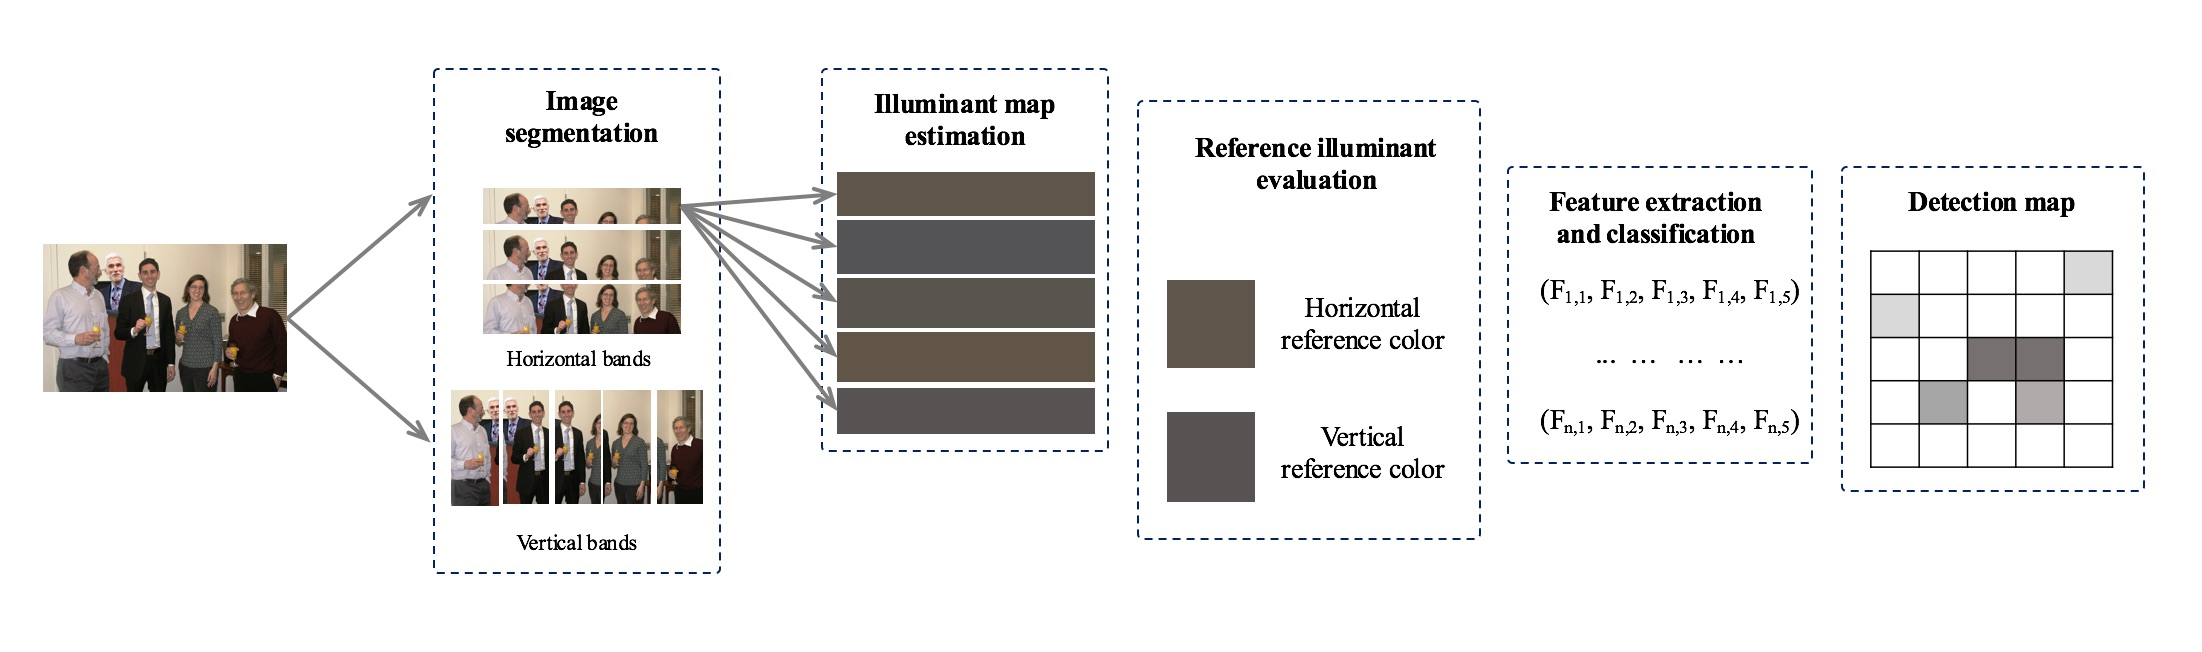
\includegraphics[width=1\textwidth]{pipeline_regions}
    \caption{Image regional splicing detection module pipeline}
    \label{fig:regionsmodulepipeline}
\end{figure}

The Figure \ref{fig:regionsmodulepipeline} summarize the module pipeline.

\subsection{Image segmentation}

In the first step of the process, the input image is segmented in order to obtain two image bands categories: horizontal and vertical bands. This kind of segmentation method is chosen because of its simplicity.

First, a band width $B_w$ and a band height $B_h$ is set. Due the fact that the segmentation has to produce overlapping bands, we set a delta factor of $\frac{1}{4}$. As a result we get overlapping stripes for a total of 25\% of their area. 

The choice of the band size is a crucial phase of the algorithm: a band too tight would fail to capture the information necessary to classify our object of interest as falsified, unlike a band too wide would capture too much additional information instead.

The choice of the overlapped area percentage makes possible a more detailed evaluation. In this way it is possible to classify the same region of the image more than once, increasing the expressive power of our final classifier.
 
In summary, let $I$ be the input image. After the segmentation process we obtain a set $B$ of bands containing all vertical and horizontal bands:

$$
B = \{V_1, \ldots, V_n, H_1, \ldots, H_m\}
$$

The dimension of $B$ is given by the sum of the number of vertical ($n$) and horizontal ($m$) bands.

\subsection{Band illuminant estimation}

The resulting image bands are now processed in order to evaluate their illuminant colors using 5 different techniques.

For this step, the Generalized Grayworld \cite{van2007edge} algorithms are used, as presented in Chapter 1. For each band, the illumination estimation is accomplished by using one of the algorithms composed of Grey-World, Max-RGB, Shades of Grey, first-order Grey-Edge and second-order Grey-Edge. Thus, we get 5 illuminant estimates for each band.
Table \ref{table:ggemethods} in Chapter 1 summarize the algorithms parameters.

$$
\forall b \in B \qquad R_a(b) = GGE_a(b) \qquad a \in \mathcal{A}
$$

where $\mathcal{A}$ is the set of the previously mentioned algorithms and $GGE_a$ is the algorithm implementation.

\subsection{Reference illuminant color estimation}

After estimating the illuminant of each horizontal/vertical band, the reference illuminant color is evaluated. Differently from Fan \emph{et al.}\cite{fan2015image}, the whole image illuminant color (obtained using the previous algorithms) is considered as reference instead of the median of all the illuminant colors extracted from all the bands of a specific direction. 

In the approach proposed in \cite{fan2015image} the reference colors were computed as follows.
 
$$
\forall a \in \mathcal{A} \qquad RV_a = median(R_a(b)) \quad \forall \; b \textrm{ vertical}
$$
$$
\forall a \in \mathcal{A} \qquad RH_a = median(R_a(b)) \quad \forall \; b \textrm{ horizontal}
$$

where $RV_a$ and $RH_a$ are the reference illuminant colors for the $a$ algorithm for vertical and horizontal direction respectively. As these two values are calculated using the median, they will be identical to one of the value of a band of that same direction.

More simply, in our case the considered reference colors are the estimation results of the 5 different algorithms over the while image. A comparison between the two estimation approaches is presented in Chapter 3.

\subsection{Feature vector estimation}

Given the two reference color for each of the two directions, a feature band for each single image band can be built.

Assuming a single light source in the image, all the evaluated illuminant will point at the same color.
Based on this assumption, a feature vector aimed at capturing illuminant colors inconsistencies can be computed.

Let $b \in B$ a single band lying on $d \in \{vertical, horizontal\}$ direction. The feature vector for $b$ will be:

\begin{equation}\label{eq:regionsfeaturevector}
f_{b} = \{m_1, m_2, m_3, m_4, m_5\}
\end{equation}
where
$$
m_i = dist(R_a(b) - RC)
$$
and $RC$ is the chosen reference color and $dist$ is the Euclidean distance function between two RGB values.

\subsection{Band classification}

Given a feature vector, a machine learning approach is used to automatically classify the band. 

After training a Support Vector Machine (SVM)\cite{bishop2007pattern} classifier with a radial basis function (RBF) kernel, we classify the resulting multidimensional feature vector $f_b$ and collect the positive output probability of this input vector, considering it as the band score.

For the SVM model training two custom dataset were specifically built containing images with single spliced band. More details about training are given in Chapter 3. 

$$
\forall \; b \in B \quad Score(b) = SVM(f_b)
$$

\subsection{Output detection map}

In order to collect all the classification outputs, a detection map is built and updated after each classifier prediction. If the result of the classification is \emph{positive} (\emph{fake}), all the pixel values that belong to the band portion in the image will be increased by the prediction score.

At the end of the process, the splicing region pixels should have greater values than the others. At this stage a color map is displayed to give a visual feedback for locating the splicing image parts.

\begin{figure}[h!]
  \centering
    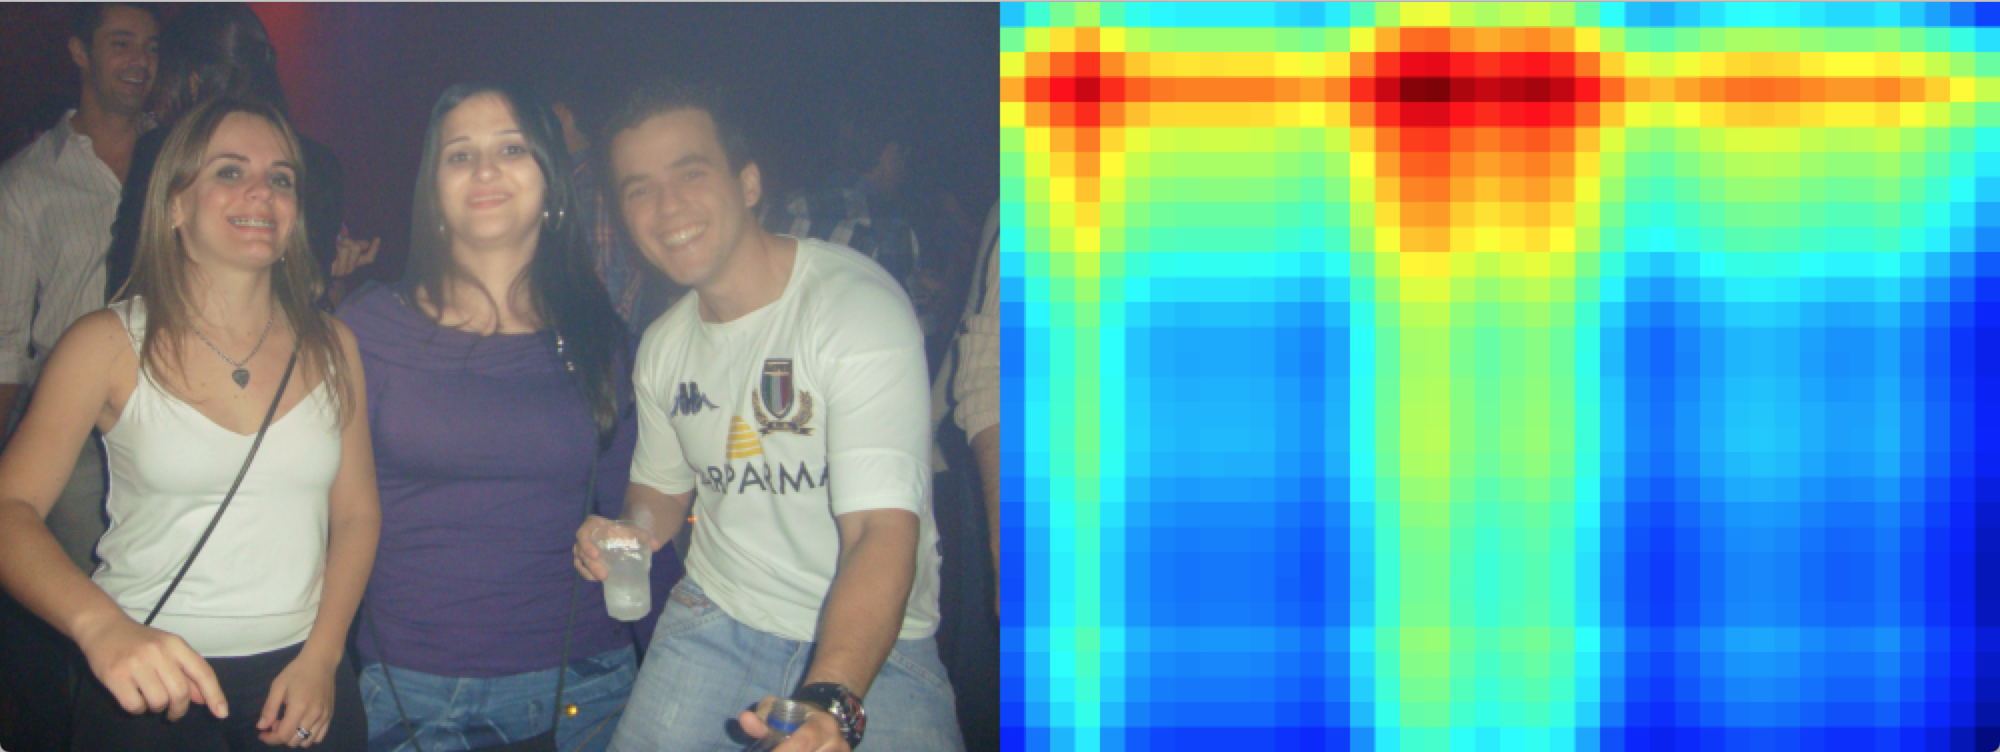
\includegraphics[width=0.9\textwidth]{detectionmapresult}
    \caption{The output detection map for an input image. The map is presented in the \emph{jet} color map representation. The map matrix intensities are in the range $[0, 1]$, and the color scheme is presented in Figure \ref{fig:colormapjet}.}\label{fig:regionsdetectionmap}
\end{figure}

\begin{figure}[h!]
  \centering
    
\includegraphics[width=0.5\textwidth]{colormap_jet}
    \caption{The \emph{jet} color map scheme. The color intensities ranges from 0 (\emph{cold} colors) to 1 (\emph{hot} colors)}
    \label{fig:colormapjet}
\end{figure}

In Figure \ref{fig:regionsdetectionmap} is presented an example of a generated detection map In this case, the splicing region consists in the woman in the middle of the scene (Figure \ref{fig:splicingmask}). As the map underlines, the more interesting region is located precisely in the middle.

Finally, the detection map is thresholded for selecting the output detected spliced regions.



